\documentclass[11pt, oneside]{article}
\usepackage{geometry}
\geometry{letterpaper}
\usepackage{graphicx}
\usepackage{amssymb}
\usepackage{amsmath}
\usepackage{tikz}
\usepackage{tikz-qtree}
\usepackage{url}
\usepackage[T1]{fontenc}

\title{SICP Exercise 3.13}
\author{Yuchong Pan}

\begin{document}
\maketitle

The box-and-pointer diagram that shows the structure created by \textbf{(define z (make-cycle (list 'a 'b 'c)))} is given as follows.

\begin{figure}[h!]
    \centering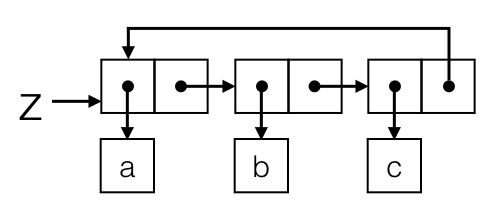
\includegraphics[width=10cm]{ex-3.13.png}
    \caption{Effect of \textbf{(define z (make-cycle (list 'a 'b 'c)))}.}
\end{figure}

If we try to compute \textbf{(last-pair z)}, the interpreter will be stuck in an infinite recursion.

\end{document}
